\section*{Der freie Fall}

Eine Masse fällt im Schwerefeld der Erde runter. Wie läuft der Fall der Masse ab?
Diese Frage kann mit dem Aufbau eines Experimentes beantwortet werden.
Dazu lassen wir eine Metallkugel aus einer vorher festgelegten Höhe zu Boden fallen.
Die Kugel benötigt für den Fall eine bestimmte Zeit $\Delta t$ die wir messen.
Um Fehler durch die Messung zu verringern, nehmen wir mehrere Zeitmessungen zu jeder
Höhenänderung vor und mitteln die Zeitspanne.
Dies wird für verschiedene Fallhöhen wiederholt. 
Die ermittelten Zeiten werden in einem Weg-Zeit-Diagramm eingetragen.


\begin{minipage}{0.5\textwidth}
%\begin{table}
	\centering
	\begin{tabular}{ccc}
		$\Delta s (\si{m})$ & $\Delta t (\si{ms})$ & $\overline{\Delta t} (\si{ms})$ \\\hline
0.1 & 129 131 130 & 130\\
0.2 & 195 200 201 & 199\\
0.3 & 241 248 244 & 244\\
0.4 & 278 285 276 & 280\\
	\end{tabular}
%	\caption{Messprotokoll für den freien Fall einer Metallkugel.}
%	\label{tab:freierfall1}
%\end{table}
\end{minipage}
\begin{minipage}{0.5\textwidth}
	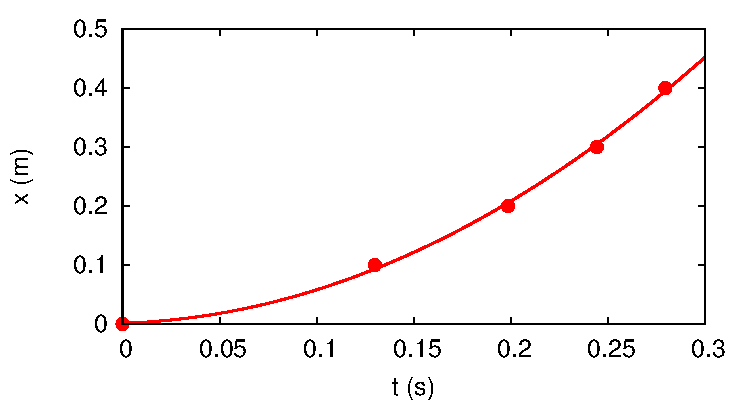
\includegraphics[width=0.95\textwidth]{./freierfall_xt.pdf}
\end{minipage}

Nun wollen wir aus dem Weg-Zeit-Diagramm ein Geschwindigkeits-Zeit-Diagramm erstellen.
Dabei gibt es einige Schwierigkeiten. Für das $v$-$t$-Diagramm wird die Momentangeschwindigkeit
benötigt. Durch die Messung kann allerdings nur eine mittlere Geschwindigkeit bestimmt werden.
Damit die mittlere Geschwindigkeit möglichst nahe an der Momentangeschwindigkeit ist, sollte eine
möglichst kleine Zeitspanne $\Delta t$ betrachtet werden.
Wir berechnen die Geschwindigkeit für die jeweils letzten \SI{10}{cm}.



\begin{minipage}{0.5\textwidth}
%\begin{table}
	\centering
	\begin{tabular}{ccc}
	$\Delta s$ &	$\Delta t (\si{s})$ & $\bar{v} (\si{m/s})$ \\\hline
%Geschwindigkeits-Zeit-Tabelle
%die letzten 10 cm
0   & 0         & 0 \\
0.1 & $\SI{130}{ms} -\SI{0}{ms}=\SI{130}{ms}$  & 0.77 \\ 
0.2 & $\SI{199}{ms} -\SI{130}{ms}=\SI{69}{ms}$  & 1.45 \\ 
0.2 & $\SI{244}{ms} -\SI{199}{ms}=\SI{45}{ms}$  & 2.22 \\ 
0.2 & $\SI{280}{ms} -\SI{244}{ms}=\SI{36}{ms}$  & 2.78 \\ 
	\end{tabular}
%	\caption{Messprotokoll für den freien Fall einer Metallkugel.}
%	\label{tab:freierfall1}
%\end{table}
\end{minipage}
\begin{minipage}{0.5\textwidth}
	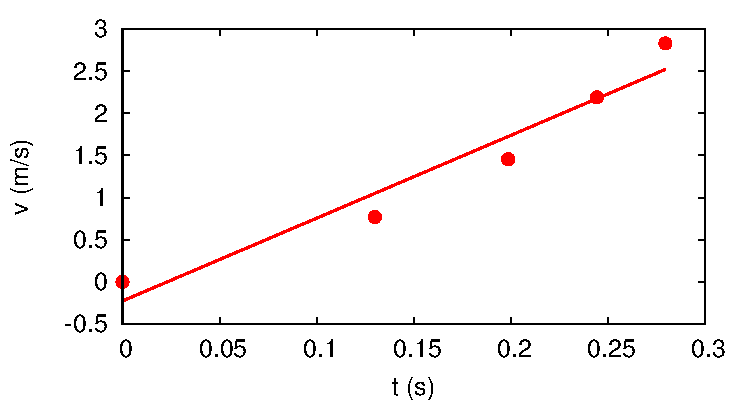
\includegraphics[width=0.95\textwidth]{./freierfall_vt.pdf}
\end{minipage}

Die berechneten Durchschnittsgeschwindigkeiten benutzen wir nun als Momentangeschwindigkeiten und tragen 
die Werte im $v$-$t$-Diagramm ein. Die Steigung der Geschwindigkeitskurve im $v$-$t$-Diagramm ist
\SI{9.92}{m/s^2}. Damit haben wir mit relativ einfachen Mitteln den Wert für die Fallbeschleunigung 
auf der Erde reproduziert und gezeigt, dass ein fallendes Objekt gleichmässig gleichförmig beschleunigt
wird, wenn es sich im Schwerefeld der Erde befindet.
Mit diesem Wissen ist es nicht mehr nötig die Momentangeschwindigkeit durch eine Durchschnittsgeschwindigkeit
zu approximieren. Stattdessen kann die Fallbeschleunigung aus dem Weg-Zeit-Diagramm bestimmt werden. 
Die Geschwindigkeit berechnet sich dann mit $v=g\cdot t$.
